\documentclass{article}

% ── NeurIPS 2026 style ───────────────────────────────────────────────────────
% Options: [preprint] for arXiv, [final] for camera-ready, default = anonymous
\usepackage{neurips_2026}
\setcitestyle{numbers,square,comma}  % [1, 2, 3]

% ── Additional packages ──────────────────────────────────────────────────────
\usepackage{amsmath,amssymb}
\usepackage{booktabs}
\usepackage{xcolor}
\usepackage{graphicx}
\usepackage{microtype}
\usepackage{enumitem}
\usepackage{pifont}
\usepackage{multirow}
\usepackage{subcaption}
\usepackage[colorlinks=true,linkcolor=blue!60!black,citecolor=green!50!black,
            urlcolor=blue!60!black]{hyperref}
\graphicspath{{figures/}}

% ── Tighten spacing (match WMF-AM) ────────────────────────────────────────
\setlength{\textfloatsep}{5pt plus 1pt minus 1pt}
\setlength{\floatsep}{5pt plus 1pt minus 1pt}
\setlength{\intextsep}{5pt plus 1pt minus 1pt}
\setlength{\abovecaptionskip}{3pt}
\setlength{\belowcaptionskip}{0pt}
\setlength{\abovedisplayskip}{4pt plus 1pt minus 1pt}
\setlength{\belowdisplayskip}{4pt plus 1pt minus 1pt}
\setlength{\parskip}{4pt plus 1pt}
\makeatletter
\renewcommand{\paragraph}{\@startsection{paragraph}{4}{\z@}%
  {0.6ex \@plus 0.2ex \@minus 0.1ex}{-1em}{\normalsize\bf}}
\renewcommand{\section}{\@startsection{section}{1}{\z@}%
  {1.2ex \@plus 0.3ex \@minus 0.2ex}{0.6ex \@plus 0.1ex}{\large\bf}}
\renewcommand{\subsection}{\@startsection{subsection}{2}{\z@}%
  {0.8ex \@plus 0.2ex \@minus 0.1ex}{0.4ex \@plus 0.1ex}{\normalsize\bf}}
\makeatother

\title{Same Brain, Different Prediction:\\How Preprocessing Choices Undermine EEG Decoding Reliability}

\author{
  Anonymous Author(s)
}

\begin{document}
\maketitle

\begin{abstract}
Electroencephalography (EEG) is a cornerstone of brain--computer interfaces and clinical neuroscience, yet deep learning models are typically trained and evaluated under a single, unreported preprocessing pipeline. We show that this practice conceals a critical reliability gap: across six datasets spanning four EEG paradigms, \textbf{up to 42\% of trial-level predictions flip} when only the preprocessing changes---a variability that standard uncertainty methods cannot detect.
We present a systematic factorial analysis of this sensitivity and make three contributions. First, a Walsh--Hadamard decomposition of the $2^7$ pipeline space reveals that preprocessing effects are predominantly additive, enabling efficient step-by-step optimization. Second, we introduce \emph{Preprocessing Uncertainty} (PU), a per-trial diagnostic that captures a dimension of instability complementary to model-based confidence. Third, we propose \emph{Normalized Adaptive PGI} (NA-PGI), a graph-structured regularizer that exploits the compositional structure of preprocessing interventions to reduce sensitivity, outperforming standard domain generalization baselines. Code and data will be released upon acceptance.
\end{abstract}

% ========== sections/introduction.tex ==========
\section{Introduction}
\label{sec:intro}

Electroencephalography (EEG) is among the lowest signal-to-noise ratio (SNR) modalities in neuroscience: single-trial cortical responses are on the order of microvolts, routinely buried under physiological and environmental noise orders of magnitude larger. Despite this, a growing body of EEG deep learning research~\citep{roy2019deep,craik2019deep} reports confident predictions---often without acknowledging a hidden source of variability that existing uncertainty methods cannot capture: \emph{the preprocessing choices made by the analyst}. Recent EEG foundation models~\citep{kostas2021bendr,jiang2024large,yang2023biot,csbrain2025,neuript2025,reve2025} learn cross-dataset representations from thousands of subjects, but their robustness to preprocessing variation remains unexamined.

Every EEG study involves at least seven independent preprocessing decisions---reference scheme, high-pass cutoff, low-pass cutoff, baseline correction, artifact attenuation, epoch rejection, and bad-channel repair---each with commonly used alternatives. These choices are rarely justified, rarely reported in full, and never tested for their impact on individual predictions. We show that this oversight has severe consequences: across six datasets spanning motor imagery, sleep staging, event-related potentials, and emotion recognition, \textbf{up to 42\% of trial-level predictions flip} when only the preprocessing changes---the model, the data, and the labels remain identical.

This finding exposes a \emph{reliability gap} in EEG deep learning. Standard uncertainty methods---softmax entropy, MC Dropout~\citep{gal2016dropout}, deep ensembles~\citep{lakshminarayanan2017simple}---capture model uncertainty but are \emph{incomplete}: they cannot detect prediction instability arising from preprocessing choices, because they hold the preprocessing fixed. A decoder may report 95\% confidence on a trial that would receive the opposite prediction under an equally valid pipeline. \emph{Preprocessing Uncertainty} (PU), a per-trial diagnostic quantifying pipeline disagreement, provides a complementary signal to standard model-based uncertainty.

We make three contributions:

\begin{enumerate}[nosep,leftmargin=*]
\item \textbf{Additivity of preprocessing sensitivity.} A Walsh--Hadamard decomposition of the $2^7$ accuracy hypercube reveals that interactions contribute $<$0.2\% of total variance in absolute terms; greedy step-by-step optimization achieves accuracy within 2.5\% of the oracle on all six datasets, making exhaustive pipeline search unnecessary.
\item \textbf{Diagnostic framework.} We define \emph{Preprocessing Uncertainty} (PU), a per-trial measure of pipeline disagreement that correlates only moderately with softmax entropy ($\rho{=}0.40$) and MC Dropout ($\rho{=}0.33$), capturing a complementary signal. Exploratory signal-level analysis reveals candidate mechanisms---e.g., high-pass filtering affects sleep staging through kurtosis reduction ($r{=}0.58$)---linking step-level sensitivity to measurable signal properties.
\item \textbf{Normalized Adaptive PGI (NA-PGI).} A graph-structured regularizer with logit-variance normalization and adaptive $\lambda$ scaling that enables a single hyperparameter ($\lambda{=}1$) to transfer across datasets, achieving up to 35\% CFR reduction while five DG baselines provide at most 3\% average improvement---echoing DomainBed~\citep{gulrajani2021search}.
\end{enumerate}

% ========== end sections/introduction.tex ==========

% ========== sections/related_work.tex ==========
\section{Related Work}
\label{sec:related}

\paragraph{EEG preprocessing pipelines.}
Standardized EEG preprocessing pipelines include PREP~\citep{bigdely2015prep}, DISCOVER-EEG~\citep{pedroni2023discover}, RELAX~\citep{bailey2023relax}, and CLEAN~\citep{clean2026}. These pipelines codify expert knowledge into fixed recipes but do not optimize for downstream decoding performance. All are MATLAB-based and rule-driven, with no mechanism to adapt to the task or model.

\paragraph{Preprocessing impact on deep learning.}
\citet{delpup2025more} trained 4,800 models across 6 tasks and found that minimal preprocessing (filtering only, no artifact removal) often outperforms complex pipelines for deep learning---suggesting that artifacts may carry useful information. \citet{kessler2025preprocessing} systematically varied filtering, referencing, and artifact correction and showed that these choices can reverse model rankings. Neither study decomposed the contribution of individual steps or compared across tasks. More broadly, shortcut learning~\citep{geirhos2020shortcut} and underspecification~\citep{damour2022underspecification} suggest that preprocessing choices may create systematic biases that models exploit without generalization, a concern amplified by recent evidence that deep networks can memorize arbitrary label assignments~\citep{zhang2021understanding}.

\paragraph{Multiverse analysis and pipeline-invariant learning.}
The ``garden of forking paths'' framework~\citep{steegen2016increasing} recognizes that analytical flexibility inflates false positives.
\citet{botvinik2020variability} showed that 70 fMRI teams reached divergent conclusions from the same data; \citet{eegmultiverse2025} computed 528 EEG pipelines but focused on statistical analysis.
\citet{li2022pipeline} proposed pipeline-invariant learning for MRI, treating pipelines as opaque domains. Recent fMRI foundation models such as NeuroSTORM~\citep{wang2026neurostorm} aim to learn preprocessing-robust representations through large-scale pretraining on 50,000+ participants, but do not quantify residual preprocessing sensitivity. This connects to the broader underspecification problem in ML~\citep{damour2022underspecification}, where multiple pipelines achieve similar validation performance but diverge at deployment. We differ from all prior work by decomposing pipelines into atomic interventions and applying factorial analysis to EEG decoding, providing a principled diagnostic for any model's preprocessing robustness.

\paragraph{EEG foundation models.}
A wave of EEG foundation models has emerged: BENDR~\citep{kostas2021bendr} applies contrastive pretraining, LaBraM~\citep{jiang2024large} scales to large multi-dataset corpora, BIOT~\citep{yang2023biot} addresses cross-modal biosignal learning, CSBrain~\citep{csbrain2025} introduces cross-scale spatiotemporal modeling across 16 datasets, NeurIPT~\citep{neuript2025} uses mixture-of-experts for heterogeneous EEG, and REVE~\citep{reve2025} pretrains on 25,000 subjects from 92 datasets. These models address cross-subject and cross-device variability but do not evaluate robustness to preprocessing choices --- the variability source we study here.

\paragraph{Domain generalization.}
Methods such as IRM~\citep{arjovsky2019invariant}, GroupDRO~\citep{sagawa2020distributionally}, and DANN~\citep{ganin2016domain} train models invariant to environment-level distribution shifts~\citep{zhou2022domain}, treating environments as unstructured groups. PGI instead leverages the known Boolean lattice structure of preprocessing interventions.

% ========== end sections/related_work.tex ==========

% ========== sections/framework.tex ==========
\section{Experimental Framework}
\label{sec:framework}

\subsection{Preprocessing as Structured Intervention}
\label{sec:interventions}

The framework uses $K{=}7$ binary preprocessing interventions, each toggling between two commonly used options selected based on their documented impact on EEG decoding~\citep{kessler2025preprocessing,delpup2025more}:

\begin{table}[h]
\centering
\caption{Seven atomic preprocessing interventions. Each has two options; all $2^7{=}128$ combinations are evaluated. ``Impact'' indicates prior evidence of effect on decoding performance.}
\label{tab:interventions}
\small
\begin{tabular}{@{}clllc@{}}
\toprule
\# & Intervention & Option A (0) & Option B (1) & Impact \\
\midrule
$a_1$ & Reference & Original & Common avg.\ ref. & Medium \\
$a_2$ & High-pass filter & 0.1\,Hz & 0.5\,Hz & High \\
$a_3$ & Low-pass filter & 45\,Hz & 30\,Hz & High \\
$a_4$ & Baseline correction & None & 200\,ms subtractive & High \\
$a_5$ & Artifact attenuation & Off & ASR~\citep{chang2020eeglab} ($\tau{=}20$) & High \\
$a_6$ & Epoch rejection & Off & Autoreject~\citep{jas2017autoreject} & Med-High \\
$a_7$ & Bad-channel repair & Off & RANSAC + interp. & Medium \\
\bottomrule
\end{tabular}
\end{table}

The 128 pipelines form a Boolean lattice---a 7-dimensional hypercube $\{0,1\}^7$---where each node is a pipeline and each edge connects two pipelines differing by exactly one intervention. This lattice has 448 undirected edges and diameter~7. For each raw EEG recording, we apply all 128 pipelines, producing 128 counterfactual versions of the same neural data.

\subsection{Metrics}

\paragraph{Counterfactual Flip Rate (CFR).}
For a trained model $f_\theta$ and a raw trial $x_i$ with label $y_i$, let $\hat{y}_i^{(p)} = \arg\max f_\theta(p(x_i))$ denote the predicted class under pipeline $p$. The CFR measures how often predictions change:
\begin{equation}
    \text{CFR} = \frac{1}{N \cdot |\mathcal{P}|} \sum_{i=1}^{N} \sum_{p \in \mathcal{P}} \mathbf{1}\!\left[\hat{y}_i^{(p)} \neq \hat{y}_i^{(p_0)}\right]
\end{equation}
where $p_0$ is a reference pipeline and $\mathcal{P}$ is the set of all 128 pipelines. We also report $\text{MaxCFR} = \max_{p,q} \frac{1}{N}\sum_i \mathbf{1}[\hat{y}_i^{(p)} \neq \hat{y}_i^{(q)}]$.

\paragraph{Per-intervention effect.}
For each intervention $a_k$, we compute the average accuracy change when toggling $a_k$ while holding all other interventions fixed:
\begin{equation}
    \Delta_k = \frac{1}{2^{K-1}} \sum_{p:\, p_k=0} \left[\text{Acc}(p \oplus e_k) - \text{Acc}(p)\right]
\end{equation}
where $p \oplus e_k$ denotes the pipeline obtained by flipping bit $k$. The absolute effect $|\Delta_k|$ measures the magnitude of sensitivity to intervention $k$, averaged over the 64 pipeline pairs that differ only on $a_k$.

\subsection{Datasets}

We use six publicly available datasets spanning distinct EEG paradigms:

\begin{table}[h]
\centering
\caption{Dataset summary. All models use EEGNet-v4~\citep{lawhern2018eegnet} with 3-fold subject-wise cross-validation.}
\label{tab:datasets}
\footnotesize
\begin{tabular}{@{}lcccccl@{}}
\toprule
Dataset & Task & Cls & Subj & Ch & Epoch & Source \\
\midrule
BCI-IV-2a~\citep{brunner2008bci} & MI & 4 & 9 & 22 & 4.0\,s & MOABB~\citep{jayaram2018moabb} \\
PhysionetMI~\citep{schalk2004bci2000} & MI & 2 & 20 & 64 & 3.0\,s & MOABB~\citep{jayaram2018moabb} \\
Sleep-EDF~\citep{kemp2000analysis} & Sleep & 5 & 15 & 2 & 30.0\,s & PhysioNet~\citep{goldberger2000physiobank} \\
BNCI2014-009 & P300 & 2 & 10 & 16 & 0.8\,s & MOABB~\citep{jayaram2018moabb} \\
Lee2019-ERP & P300 & 2 & 10 & 62 & 1.0\,s & MOABB~\citep{jayaram2018moabb} \\
SEED-IV & Emotion & 4 & 15 & 62 & 4.0\,s & BCMI~\citep{zheng2019emotionmeter} \\
\bottomrule
\end{tabular}
\end{table}

\paragraph{Protocol.}
\textbf{Sensitivity analysis} (Section~\ref{sec:results}): train EEGNet on a single anchor pipeline $p_0$, evaluate on all 128 pipelines to isolate preprocessing sensitivity from training effects. Per-intervention effects $\Delta_k$ average over 64 pipeline pairs and are anchor-independent. \textbf{Mitigation} (Section~\ref{sec:napgi}): NA-PGI and all baselines train on all pipeline views with matched budgets (50 epochs, same optimizer/backbone, 3-fold CV split before preprocessing) and are evaluated on all 128 pipelines.

\paragraph{Computational cost.}
All preprocessing uses MNE-Python~\citep{gramfort2013mne}; generating 128 variants takes ${\sim}10$ min/subject (CPU), and ERM training takes ${\sim}1$ GPU-hour/dataset on an A100.

% ========== end sections/framework.tex ==========

% ========== sections/results.tex ==========
\section{Results}
\label{sec:results}

\subsection{Preprocessing Sensitivity is Real and Task-Specific}

Table~\ref{tab:cfr} summarizes baseline sensitivity across all six datasets. On motor imagery (BCI-IV-2a), a mean of \textbf{42.4\% of predictions flip} across 128 pipelines. Emotion recognition (SEED-IV) shows similarly high sensitivity (35.8\%). Even on high-accuracy tasks, sensitivity is nontrivial: 9.6\% for sleep staging and 2.6--4.1\% for P300/ERP.

\begin{table}[t]
\centering
\caption{Preprocessing sensitivity across tasks (ERM-single, EEGNet, 3-fold CV). CFR = mean fraction of test trials whose prediction changes across 128 pipelines.}
\label{tab:cfr}
\small
\begin{tabular}{@{}lccc@{}}
\toprule
Dataset & Channels & Mean Acc.\ (\%) & CFR (\%) \\
\midrule
BCI-IV-2a (MI, 4-cls) & 22 & 37.6 & \textbf{42.4} \\
SEED-IV (Emotion, 4-cls) & 62 & 31.9 & 35.8 \\
PhysionetMI (MI, 2-cls) & 64 & 57.7 & 21.7 \\
Sleep-EDF (Sleep, 5-cls) & 2 & 85.6 & 9.6 \\
Lee2019-ERP (ERP, 2-cls) & 62 & 84.1 & 4.1 \\
P300 (ERP, 2-cls) & 16 & 83.4 & 2.6 \\
\bottomrule
\end{tabular}
\end{table}

Sensitivity inversely correlates with task accuracy (Figure~\ref{fig:cfr_summary}): when the decoder is least confident (BCI-IV-2a, 37.6\%), preprocessing has the most influence. The best--worst pipeline gap reaches 24.0 percentage points on BCI-IV-2a (49.7\% vs.\ 25.7\%)---meaning the \emph{choice of preprocessing alone} determines nearly a quarter of the accuracy range.

\begin{figure}[t]
    \centering
    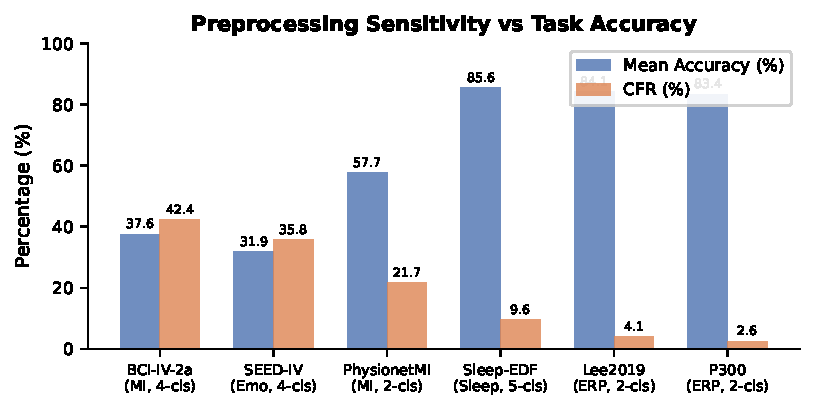
\includegraphics[width=0.75\linewidth]{figures/fig1_cfr_summary.pdf}
    \caption{Preprocessing sensitivity (CFR) inversely correlates with task accuracy across all six datasets. Preprocessing choices matter most when the model is least confident.}
    \label{fig:cfr_summary}
\end{figure}

Which interventions drive this sensitivity differ across tasks (Figure~\ref{fig:heatmap}): epoch rejection dominates BCI-IV-2a ($|\Delta|{=}20.9\%$), while high-pass filtering dominates Sleep-EDF ($4.8\%$) and P300 ($2.8\%$). Pairwise Spearman rank correlations of intervention importance are low (mean $\rho{=}0.274$; Appendix Table~\ref{tab:spearman}), confirming that rankings are largely non-transferable across tasks.

\begin{figure}[t]
    \centering
    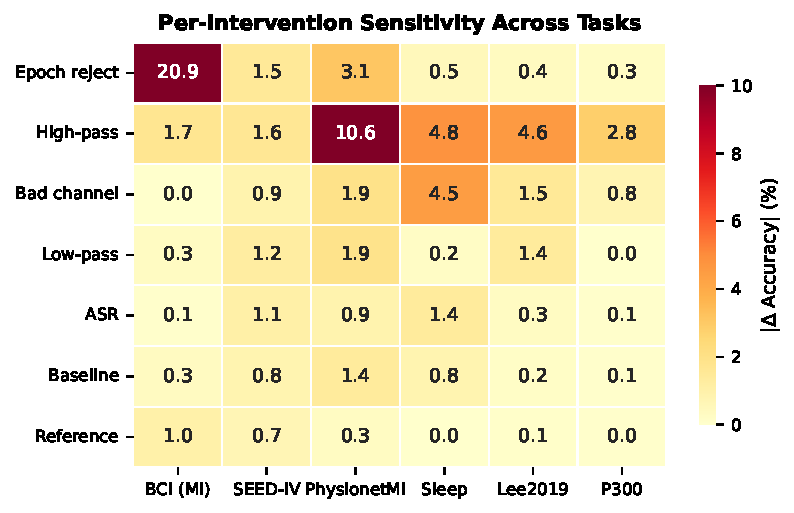
\includegraphics[width=0.65\linewidth]{figures/fig2_intervention_heatmap.pdf}
    \caption{\textbf{Preprocessing sensitivity is task-specific.} Each cell shows $|\Delta_k|$ (\%) when toggling one intervention, averaged over 64 pipeline pairs across all six datasets. Motor imagery is dominated by epoch rejection; sleep staging and ERP tasks by high-pass filtering.}
    \label{fig:heatmap}
\end{figure}

\subsection{Sensitivity is Additive: Walsh--Hadamard Interaction Spectrum}

Prior multiverse studies report marginal effects but do not characterize whether preprocessing steps \emph{interact}. We apply a Walsh--Hadamard decomposition~\citep{rao1999walsh} to the $2^7$ accuracy hypercube, partitioning total variance into main effects (order 1), pairwise interactions (order 2), and higher-order terms.

\begin{table}[t]
\centering
\caption{Walsh--Hadamard variance decomposition of per-pipeline accuracy across all six datasets. In absolute terms, interactions (order $\geq$2) contribute $<$0.2\% of total variance; however, when measured relative to non-mean variance, interaction shares range from 0.6\% (BCI) to 54\% (SEED-IV). Despite this, greedy step-by-step optimization achieves accuracy within 2.5\% of the oracle on all six datasets (see text).}
\label{tab:wht}
\small
\begin{tabular}{@{}lcccc@{}}
\toprule
Dataset & Order 0 (mean) & \textbf{Order 1 (main)} & Order 2 (pairs) & Order 3+ \\
\midrule
BCI-IV-2a & 92.8\% & \textbf{7.2\%} & $<$0.1\% & $<$0.01\% \\
PhysionetMI & 99.0\% & \textbf{0.9\%} & 0.1\% & $<$0.1\% \\
SEED-IV & 99.7\% & \textbf{0.1\%} & 0.1\% & 0.1\% \\
Sleep-EDF & 99.8\% & \textbf{0.2\%} & $<$0.1\% & $<$0.01\% \\
Lee2019-ERP & 99.9\% & \textbf{0.1\%} & $<$0.1\% & $<$0.01\% \\
P300 & 100.0\% & \textbf{$<$0.1\%} & $<$0.01\% & $<$0.01\% \\
\bottomrule
\end{tabular}
\end{table}

The result (Table~\ref{tab:wht}) shows that across all six datasets, \textbf{interactions contribute $<$0.2\% of total variance in absolute terms}. However, because the order-0 mean dominates total variance (92--100\%), the picture changes when measured relative to non-mean variance: the interaction share of non-mean variance ranges from 0.6\% on BCI-IV-2a to 54\% on SEED-IV. On SEED-IV, main effects and interactions are comparable in magnitude once the grand mean is removed.

The practical question is whether these interactions are large enough to require joint optimization. We validate this with a greedy step-by-step optimization experiment across all six datasets: the greedy-optimal pipeline achieves accuracy within 2.5\% of the oracle best-of-128 on every dataset, with SEED-IV showing the largest gap (2.5\%) and Lee2019-ERP the smallest (0.4\%). \textbf{Step-wise tuning is thus a strong practical approximation under the binary intervention design studied here}---tuning each intervention in isolation captures most of the achievable improvement, even on datasets where the relative interaction share is substantial. This additivity may not extend to continuous preprocessing parameters (e.g., HPF cutoff sweeps), where~\citet{kessler2025preprocessing} reported meaningful interactions.

Exploratory signal-level analysis suggests candidate mechanistic pathways for why specific interventions matter: high-pass filtering correlates with sleep staging accuracy through kurtosis reduction, while epoch rejection affects motor imagery through training-set composition changes (full analysis in Appendix~\ref{app:signal}).

\subsection{Pipeline Disagreement as Epistemic Uncertainty}

Given that preprocessing changes predictions without changing the data, a natural question is whether this instability can be quantified per trial.
\emph{Preprocessing Uncertainty} (PU) for a trial $x_i$ is defined as:
$\text{PU}(x_i) = 1 - \max_{c} \frac{1}{|\mathcal{P}|}\sum_{p} \mathbf{1}[\hat{y}_i^{(p)} = c]$,
ranging from 0 (all pipelines agree) to $1-1/|\mathcal{C}|$ (uniform disagreement). PU captures analyst degrees of freedom rather than model stochasticity.

We evaluate PU as an error detector using standard UQ benchmarks (for a comprehensive review of uncertainty quantification techniques, see~\citet{abdar2021review}). Table~\ref{tab:pu} summarizes PU error-detection performance and its correlation with model-based uncertainty across three datasets. On PhysionetMI, PU achieves AUROC 0.712 for error detection, comparable to softmax entropy (0.764) and MC Dropout (0.721). PU correlates only moderately with model-based methods (mean $\rho{=}0.40$ vs.\ softmax, $\rho{=}0.33$ vs.\ MC Dropout across three datasets), substantially lower than the mutual correlation between softmax and MC Dropout ($\rho{=}0.55$). The degree of complementarity is dataset-dependent: on BCI-IV-2a, PU is nearly independent ($\rho{=}0.30$), while on PhysionetMI, correlation is moderate ($\rho{=}0.52$). On PhysionetMI, combining PU with softmax yields AUROC 0.783---exceeding either alone and demonstrating complementarity; on BCI-IV-2a, the combination does not improve over softmax alone, suggesting that PU's value is greatest when preprocessing sensitivity is high. Full calibration and selective prediction results are in the appendix.

\begin{table}[t]
\centering
\caption{PU as error detector: AUROC for error detection and Spearman correlation with model-based uncertainty across three datasets (mean over 3 folds).}
\label{tab:pu}
\small
\begin{tabular}{@{}lccccc@{}}
\toprule
Dataset & PU AUROC & Softmax AUROC & MC AUROC & $\rho$(PU, Soft) & $\rho$(Soft, MC) \\
\midrule
BCI-IV-2a & 0.548 & 0.636 & 0.604 & 0.298 & 0.625 \\
PhysionetMI & 0.712 & 0.764 & 0.721 & 0.519 & 0.695 \\
SEED-IV & 0.528 & 0.525 & 0.538 & 0.379 & 0.334 \\
\bottomrule
\end{tabular}
\end{table}

Oracle pipeline selection reveals substantial performance headroom: on BCI-IV-2a, keeping only the top 50\% of pipelines improves accuracy by +10.4\% (Appendix Table~\ref{tab:selective}). Combined with the additivity result, this implies that a practitioner who tunes each preprocessing step independently on a validation set should approach the oracle bound.

% ========== end sections/results.tex ==========

% ========== sections/pgi.tex ==========
\section{Mitigation: Normalized Adaptive PGI}
\label{sec:napgi}

Given that preprocessing sensitivity is real, additive, and task-specific, we ask: can we train decoders that are less sensitive to preprocessing choices? We propose \emph{Normalized Adaptive Pipeline Generator Invariance} (NA-PGI), a plug-in training objective that penalizes prediction drift across atomic preprocessing changes with two key innovations for cross-dataset robustness.

\subsection{Base Method: Pipeline Generator Invariance}

The 128 pipelines form a Boolean lattice where each edge toggles exactly one of the $K{=}7$ atomic interventions. This graph-structured regularization is inspired by the observation that preprocessing interventions have a natural compositional structure: each edge in the lattice corresponds to toggling exactly one preprocessing step, making edge-level consistency a minimal and interpretable invariance constraint. PGI adds a consistency loss on these edges: for centered logits $\bar{z}_i^{(p)} = z_i^{(p)} - \frac{1}{C}\sum_c z_{i,c}^{(p)}$, the base PGI loss is:
\begin{equation}
    \mathcal{L}_{\text{PGI}} = \frac{1}{|E|} \sum_{(p,q) \in E} w_{(p,q)} \cdot \frac{1}{B}\sum_{i=1}^{B}\|\bar{z}_i^{(p)} - \bar{z}_i^{(q)}\|_2^2
\end{equation}

\subsection{Problem: Loss Scale Mismatch}

Na\"ive PGI with a fixed $\lambda$ fails across datasets because \textbf{logit magnitudes vary by up to 50$\times$} depending on channel count and task complexity. A $\lambda$ tuned for BCI-IV-2a (22 channels, small logits) causes collapse on SEED-IV (62 channels, large logits), as the PGI penalty overwhelms the supervised loss.

\subsection{Solution: NA-PGI}

We introduce two complementary fixes, each addressing a different failure mode:

\paragraph{Fix 1: Loss normalization (scale invariance).}
We divide the PGI loss by the \emph{detached} logit variance, making the penalty scale-invariant:
\begin{equation}
    \mathcal{L}_{\text{N-PGI}} = \frac{\mathcal{L}_{\text{PGI}}}{\text{sg}[\text{Var}(\bar{z})] + \epsilon}
\end{equation}
where $\text{sg}[\cdot]$ denotes stop-gradient (preventing the model from inflating logits to trivially minimize the ratio). This ensures that $\lambda{=}1$ carries the same semantic meaning regardless of dataset: ``the invariance penalty should be comparable in magnitude to the cross-entropy loss.''

\paragraph{Fix 2: Adaptive $\lambda$ (collapse prevention).}
We modulate $\lambda$ based on the running evaluation CFR:
\begin{equation}
    \lambda_{\text{eff}} = \lambda \cdot \text{clamp}\!\left(\frac{\overline{\text{CFR}}}{\tau}, 0.01, 5.0\right)
\end{equation}
where $\overline{\text{CFR}}$ is an exponential moving average of the validation CFR and $\tau{=}0.15$ is a target CFR. When CFR is high (model is sensitive), $\lambda$ is boosted; when CFR drops toward zero (collapse risk), $\lambda$ is automatically reduced, allowing the supervised loss to recover. The EMA is initialized to $\tau$ so that $\lambda$ starts at its base value.

\paragraph{Why both fixes are necessary.} Our ablation (Table~\ref{tab:ablation}) shows that normalization alone still collapses on 2/3 datasets (the gradient landscape remains unstable without the dynamic safety net), while adaptive-only without normalization yields inconsistent results across datasets (the raw loss scale still varies). Only the combination provides robust, cross-dataset performance with a single $\lambda{=}1$.

\subsection{Results}

We compare NA-PGI against six baselines on three high-CFR datasets (Table~\ref{tab:main}).

\begin{table}[t]
\centering
\caption{CFR (fraction) across methods on 128-pipeline evaluation. Domain generalization baselines in our simplified implementations (GroupDRO, IRM) provide marginal improvement, consistent with DomainBed~\citep{gulrajani2021search}. NA-PGI achieves the best average CFR reduction.}
\label{tab:main}
\small
\begin{tabular}{@{}lccc|c@{}}
\toprule
Method & BCI-IV-2a & PhysionetMI & SEED-IV & Avg.\ $\Delta$ \\
\midrule
ERM-single & 0.424 & 0.217 & 0.358 & --- \\
ERM-mixed & 0.424 ($-$0\%) & 0.221 ($-$2\%) & 0.323 (+10\%) & +3\% \\
GroupDRO & 0.412 (+3\%) & 0.223 ($-$3\%) & 0.332 (+7\%) & +2\% \\
IRM & 0.412 (+3\%) & 0.228 ($-$5\%) & 0.314 (+12\%) & +3\% \\
Consistency & 0.418 (+2\%) & \textbf{0.178} (+18\%) & 0.311 (+13\%) & +11\% \\
CORAL & 0.419 (+1\%) & 0.252 ($-$16\%) & 0.274 (+24\%) & +3\% \\
\textbf{NA-PGI} & 0.406 (+4\%) & 0.187 (+14\%) & \textbf{0.233} (+35\%) & \textbf{+18\%} \\
\bottomrule
\end{tabular}
\end{table}

Our analysis yields three insights regarding domain generalization under preprocessing shifts:

\paragraph{The DomainBed phenomenon in EEG.}
Consistent with large-scale DG meta-analyses~\citep{gulrajani2021search}, our simplified implementations of GroupDRO and IRM yield only +2--3\% average improvement over ERM-mixed. Canonical implementations with stable group tracking may perform differently (see Appendix for implementation details).

\paragraph{Feature-space alignment instability.}
Our simplified CORAL~\citep{sun2016deep} implementation exhibits instability: +24\% on SEED-IV but $-$16\% on PhysionetMI. We hypothesize that enforcing feature-space alignment may be overly aggressive for EEG, though this may also reflect our simplified implementation (feature-mean divergence rather than full covariance).

\paragraph{Prediction-space consistency vs.\ NA-PGI.}
In contrast, regularizing the \emph{output} prediction space proves much safer. Consistency regularization---which treats all 128 pipelines as independent, equally distant domains---achieves a robust +11\% average, particularly on PhysionetMI (+18\%). NA-PGI achieves the highest overall efficacy (+18\% average), largely driven by a substantial +35\% on SEED-IV. While Consistency treats pipelines as a flat set, NA-PGI leverages the topological structure of the intervention lattice, penalizing drift along atomic edges rather than across arbitrary pipeline pairs. Combined with adaptive scale normalization, this achieves strong invariance without sacrificing stability on high-dimensional data. NA-PGI uses a single $\lambda{=}1$ without per-dataset tuning.

\paragraph{Multi-seed stability (5 seeds).} On PhysionetMI (64 channels), NA-PGI is highly stable across 5 random seeds (CFR $0.135 \pm 0.037$), with all seeds showing substantial improvement over ERM (0.217). SEED-IV (62 channels) achieves the largest mean reduction ($0.114 \pm 0.065$ vs.\ ERM 0.358, $-68\%$), though variability is high and one seed exhibits fold-level collapse. On BCI-IV-2a (22 channels, 4-class), improvement is marginal ($0.410 \pm 0.056$ vs.\ ERM 0.424, $-3\%$) with one seed showing fold-level collapse. We analyze the failure mode in Section~\ref{sec:discussion}.

\paragraph{Accuracy--CFR tradeoff.} Table~\ref{tab:acc_cfr} reports both accuracy and CFR for the main methods. NA-PGI maintains accuracy within 1 percentage point of ERM on PhysionetMI and SEED-IV while reducing CFR by 14--35\%. On BCI-IV-2a, the accuracy cost is larger ($-$7.1\,pp), reflecting the representational capacity constraint on low-channel data. This tradeoff is acceptable when preprocessing robustness is prioritized over peak single-pipeline performance.

\begin{table}[t]
\centering
\caption{Mean accuracy (\%) and CFR (\%) for key methods. NA-PGI achieves the best CFR reduction with modest accuracy cost.}
\label{tab:acc_cfr}
\small
\begin{tabular}{@{}l|cc|cc|cc@{}}
\toprule
 & \multicolumn{2}{c|}{BCI-IV-2a} & \multicolumn{2}{c|}{PhysionetMI} & \multicolumn{2}{c}{SEED-IV} \\
Method & Acc & CFR & Acc & CFR & Acc & CFR \\
\midrule
ERM-single & 37.6 & 42.4 & 57.7 & 21.7 & 31.9 & 35.8 \\
Consistency & 38.8 & 41.8 & 57.1 & 17.8 & 32.3 & 31.1 \\
NA-PGI & 30.5 & 40.6 & 56.9 & 18.7 & 33.7 & 23.3 \\
\bottomrule
\end{tabular}
\end{table}

\begin{table}[t]
\centering
\caption{Ablation study. Both normalization and adaptive $\lambda$ are necessary. Normalize-only collapses on 2/3 datasets; adaptive-only is inconsistent across datasets. Only NA-PGI (both) provides robust cross-dataset improvement.}
\label{tab:ablation}
\small
\begin{tabular}{@{}cclccc@{}}
\toprule
Norm. & Adapt. & Config & BCI & Phys. & SEED \\
\midrule
\ding{55} & \ding{55} & Old PGI ($\lambda{=}5$) & 0.337 & 0.235 & \textit{collapse} \\
\ding{51} & \ding{55} & Normalize-only & 0.406 & 0.214 & \textit{collapse} \\
\ding{55} & \ding{51} & Adaptive-only & 0.395 & 0.126 & 0.306 \\
\ding{51} & \ding{51} & \textbf{NA-PGI} & 0.406 & 0.187 & \textbf{0.233} \\
\bottomrule
\end{tabular}
\end{table}

% ========== end sections/pgi.tex ==========

% ========== sections/discussion.tex ==========
\section{Discussion}
\label{sec:discussion}

\paragraph{Relation to concurrent work.}
\citet{kessler2025preprocessing} reported meaningful interactions for continuous preprocessing parameters in ERP decoding; our binary design finds interactions small in absolute terms ($<$0.2\%) but up to 54\% of non-mean variance on SEED-IV---the practical implication is identical: \emph{validate preprocessing choices for each task.} \citet{delpup2025more} compared preprocessing \emph{levels} across six tasks; we decompose individual steps and explain \emph{why} they matter. \citet{delorme2023eeg} showed that ERP significance benefits little from complex preprocessing; we extend this to deep learning decoders and provide both a diagnostic (PU) and a mitigation method (NA-PGI). The underspecification framework of \citet{damour2022underspecification} provides a complementary perspective: our 128 pipelines represent a concrete instance of the ``pipeline multiplicity'' problem, where many equally valid preprocessing choices lead to divergent predictions. Our simplified implementations of GroupDRO, IRM, and CORAL (Table~\ref{tab:main}) provide at most 3\% average CFR reduction---echoing DomainBed's~\citep{gulrajani2021search} observation that ERM is hard to beat. One structural advantage of NA-PGI is that it exploits the compositional structure of preprocessing interventions through edge-level consistency, rather than treating pipelines as opaque domains; recent DG surveys~\citep{zhou2022domain} suggest that domain structure, when available, should be incorporated into invariance constraints, and our Boolean lattice provides exactly this structure.

\paragraph{Limitations and failure modes.}
Our study has several boundaries that should guide interpretation and future work.
\emph{Method robustness:} NA-PGI can exhibit optimization instability on low-channel data. On the 22-channel BCI-IV-2a, one of five seeds produced representational collapse (CFR$\to$0), likely due to over-compression of sparse discriminative signals when enforcing invariance across 128 pipeline variants. We recommend NA-PGI primarily for high-density EEG ($\geq$60 channels), where Consistency regularization is a safer alternative for low-channel regimes.
\emph{Factorial design:} The Walsh--Hadamard additivity analysis is verified only on binary interventions (e.g., ``apply ASR or not''); continuous preprocessing parameters such as precise bandpass cutoffs or artifact rejection thresholds may harbor non-linear effects not captured by our binary design, as suggested by~\citet{kessler2025preprocessing}.
\emph{Generalization:} All results use EEGNet and ShallowNet; sensitivity patterns may differ for larger models or EEG foundation models~\citep{kostas2021bendr,jiang2024large,csbrain2025,neuript2025,reve2025,wang2026neurostorm}---applying our CFR framework to these models is a natural next step. Spearman $\rho$ over 7 items has limited statistical power, and the signal-level analysis is correlational rather than causal.

\paragraph{Cross-architecture validation.}
To verify that preprocessing sensitivity is not an artifact of EEGNet, we repeat the ERM-single evaluation with ShallowNet~\citep{schirrmeister2017deep} (Table~\ref{tab:shallow}). CFR values are consistent across architectures (within 6 percentage points), confirming that CFR reflects data-level variability rather than architecture-specific artifacts.

\begin{table}[h]
\centering
\caption{CFR and accuracy under ERM-single for EEGNet vs.\ ShallowNet on three high-CFR datasets. Preprocessing sensitivity is consistent across architectures.}
\label{tab:shallow}
\small
\begin{tabular}{@{}lcccc@{}}
\toprule
Dataset & \multicolumn{2}{c}{EEGNet} & \multicolumn{2}{c}{ShallowNet} \\
\cmidrule(lr){2-3} \cmidrule(lr){4-5}
 & Acc & CFR & Acc & CFR \\
\midrule
BCI-IV-2a & 37.6 & 42.4 & 33.0 & 47.8 \\
PhysionetMI & 57.7 & 21.7 & 56.8 & 22.7 \\
SEED-IV & 31.9 & 35.8 & 31.5 & 37.5 \\
\bottomrule
\end{tabular}
\end{table}

\paragraph{Practical recommendations.}
\begin{enumerate}[nosep,leftmargin=*]
\item \textbf{Optimize preprocessing step-by-step.} Greedy step-by-step tuning achieves accuracy within 2.5\% of the oracle on all six datasets; exhaustive pipeline search is unnecessary.
\item \textbf{Consider NA-PGI for high-channel recordings.} NA-PGI provides out-of-the-box preprocessing robustness with $\lambda{=}1$ on 60+ channel setups. For low-channel configurations, Consistency regularization is a safer alternative.
\item \textbf{Report PU alongside accuracy.} A model with 80\% accuracy and 40\% CFR is fundamentally different from one with 80\% accuracy and 2\% CFR; PU makes this distinction visible at zero additional training cost.
\end{enumerate}

\paragraph{Why does NA-PGI fail on low-channel data?}
We hypothesize two contributing factors. First, with only 22 channels (BCI-IV-2a), the feature space has limited capacity to simultaneously encode task-discriminative information and maintain cross-pipeline consistency across 128 variants---an \emph{information bottleneck} that forces the model to sacrifice accuracy for invariance. Second, the EMA-based adaptive $\lambda$ controller exhibits a \emph{dynamic lag}: when CFR drops abruptly (indicating onset of collapse), the controller cannot relax $\lambda$ fast enough to prevent the supervised loss from being overwhelmed. This suggests that a more responsive controller (e.g., per-step rather than per-epoch adaptation) could improve stability on low-channel data.

\paragraph{Future directions.}
Three extensions would strengthen the contribution.
First, extending the factorial analysis to continuous preprocessing parameters (e.g., high-pass cutoff at 0.01/0.1/0.3/0.5/1.0\,Hz) would test whether the additivity finding holds beyond binary choices.
Second, applying our CFR framework as a robustness diagnostic for EEG foundation models~\citep{csbrain2025,neuript2025,reve2025} would reveal whether large-scale pretraining truly eliminates preprocessing sensitivity or merely reduces it.
Third, combining PU with model-based uncertainty in a principled Bayesian framework, rather than the current min-max normalization, could yield a more calibrated composite uncertainty estimate.

\paragraph{Broader impact and conclusion.}
Preprocessing sensitivity has immediate implications for clinical EEG, where prediction reliability is safety-critical: brain-computer interfaces~\citep{blankertz2007bci} and seizure detection systems rely on consistent predictions, and deploying a decoder without reporting its preprocessing sensitivity risks undetected failure modes. Our factorial characterization, the PU diagnostic, and NA-PGI provide both diagnostic tools and practical mitigation for building more reliable EEG-based systems. Code and preprocessed data will be released upon acceptance.

% ========== end sections/discussion.tex ==========


\bibliographystyle{unsrtnat}
\bibliography{references}

\newpage
\appendix
% ========== sections/appendix.tex ==========
\section{Additional Results}
\label{app:additional}

\subsection{Spearman Rank Correlations of Intervention Importance}

\begin{table}[h]
\centering
\caption{Spearman rank correlations of intervention importance on three representative datasets (BCI-IV-2a, Sleep-EDF, P300).}
\label{tab:spearman}
\small
\begin{tabular}{@{}lccc@{}}
\toprule
 & BCI-IV-2a & Sleep-EDF & P300 \\
\midrule
BCI-IV-2a & 1.000 & $-$0.214 & +0.214 \\
Sleep-EDF & & 1.000 & \textbf{+0.821} \\
P300 & & & 1.000 \\
\midrule
\multicolumn{4}{l}{Mean pairwise $\rho = 0.274$} \\
\bottomrule
\end{tabular}
\end{table}

\subsection{Signal-Level Correlates}
\label{app:signal}

For one representative subject per dataset, we compute trial-level signal statistics---amplitude, channel variance dispersion, low-frequency power, trial-level maximum, and kurtosis---over 100 sampled trials and examine how interventions alter these features and how those alterations relate to accuracy.

\begin{table}[h]
\centering
\caption{Signal--accuracy correlations ($r$) and per-intervention associations on three representative datasets (one representative subject, 100 trials per dataset). Note: these are correlational, not causal.}
\label{tab:mediation}
\small
\begin{tabular}{@{}llcll@{}}
\toprule
Dataset & Top correlate & $r$ & Dominant intervention & Mediating mechanism \\
\midrule
BCI-IV-2a & Amplitude & +0.19 & Epoch rejection & $\Delta$\,lf\_power \\
Sleep-EDF & Ch.\ var.\ disp. & +0.60 & High-pass filter & $\Delta$\,kurtosis ($-$0.46) \\
P300 & Kurtosis & +0.38 & High-pass filter & $\Delta$\,kurtosis ($-$0.12) \\
\bottomrule
\end{tabular}
\end{table}

\begin{itemize}
    \item \textbf{Sleep staging:} Accuracy correlates strongly with channel variance dispersion ($r{=}+0.60$) and kurtosis ($r{=}+0.58$). High-pass filtering at 0.5\,Hz (vs.\ 0.1\,Hz) significantly reduces kurtosis ($\Delta{=}-0.46$), which in turn reduces accuracy by 4.8\%.
    \item \textbf{P300:} Kurtosis correlates with accuracy ($r{=}+0.38$), and high-pass filtering reduces kurtosis ($\Delta{=}-0.12$), reducing accuracy by 2.8\%.
    \item \textbf{Motor imagery:} Epoch rejection operates through a different pathway: removing outlier trials changes the training distribution's low-frequency power. The signal-accuracy correlation is weaker ($r{=}+0.19$), suggesting that for MI, the effect is more about \emph{which data is kept} than \emph{how the signal is transformed}.
\end{itemize}

\subsection{Oracle Pipeline Selection}

\begin{table}[h]
\centering
\caption{Selective pipeline prediction (oracle upper bound) on three representative datasets: accuracy when retaining only the top-$K$\% pipelines by per-pipeline test accuracy.}
\label{tab:selective}
\small
\begin{tabular}{@{}lccccc@{}}
\toprule
Dataset & All 128 & Top 75\% & Top 50\% & Top 25\% & Top 10\% \\
\midrule
BCI-IV-2a & 37.6 & 41.2 & \textbf{48.0} & 49.4 & 49.7 \\
Sleep-EDF & 85.6 & 87.3 & \textbf{88.4} & 89.4 & 89.6 \\
P300 & 83.4 & 84.0 & \textbf{84.8} & 85.0 & 85.3 \\
\bottomrule
\end{tabular}
\end{table}

\subsection{Signed Intervention Effects}

Figure~\ref{fig:signed} shows the \emph{signed} per-intervention effects, revealing that the same intervention can have opposite effects across tasks. For example, ASR has a weakly positive effect on BCI-IV-2a but a negative effect on Sleep-EDF.

\begin{figure}[h]
    \centering
    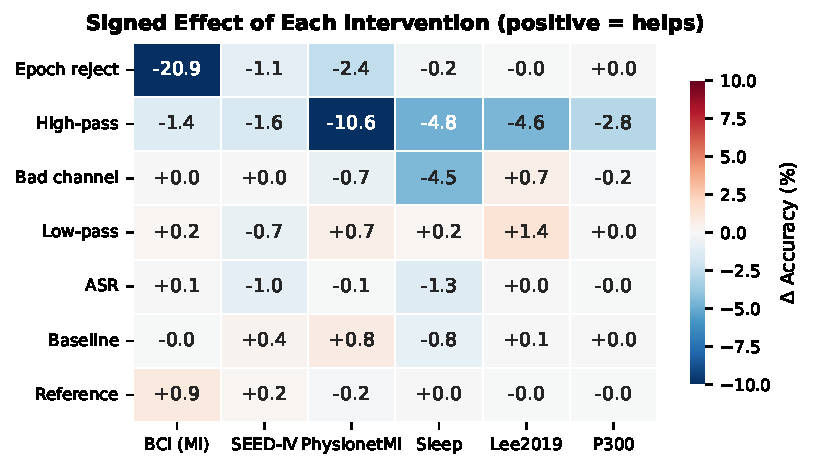
\includegraphics[width=0.65\linewidth]{figures/fig3_signed_effects.pdf}
    \caption{Signed effect ($\Delta_k$, \%) of each intervention across all six datasets. Positive values indicate that enabling the intervention improves accuracy. Note the sign flips for ASR and bad-channel repair across tasks.}
    \label{fig:signed}
\end{figure}

\subsection{PGI Implementation Details}

PGI adds approximately 10 lines to a standard training loop:
{\small
\begin{verbatim}
logits = decoder(views.flatten(0,1)).view(B, V, C)
sup = F.cross_entropy(logits.reshape(B*V,C),
                      y.repeat_interleave(V))
z = logits - logits.mean(dim=-1, keepdim=True)
edge_loss = ((z[:,src]-z[:,dst]).pow(2).sum(-1)*w).mean()
loss = sup + lam * edge_loss
\end{verbatim}
}
where \texttt{src}, \texttt{dst} are pre-computed Hasse edge indices and \texttt{w} contains per-intervention weights. For NA-PGI, add logit-variance normalization (\texttt{/ z.detach().pow(2).mean()}) and adaptive $\lambda$ modulation.

\subsection{NA-PGI Stability Across Seeds}

\begin{table}[h]
\centering
\caption{NA-PGI CFR across 5 random seeds. PhysionetMI is highly stable (std$=$0.037); SEED-IV shows high variability but consistent improvement over ERM (0.358). BCI-IV-2a shows marginal improvement with occasional fold-level collapse. $^\dagger$At least one fold collapsed (CFR$\to$0); early-stopping may or may not preserve a non-degenerate checkpoint.}
\label{tab:seeds}
\small
\begin{tabular}{@{}lcccccc@{}}
\toprule
Dataset & S42 & S43 & S44 & S45 & S46 & Mean$\pm$Std \\
\midrule
BCI-IV-2a (22ch) & 0.406 & 0.460 & 0.438 & 0.442 & 0.304$^\dagger$ & 0.410$\pm$0.056 \\
PhysionetMI (64ch) & 0.187 & 0.140 & 0.155 & 0.079 & 0.114 & 0.135$\pm$0.037 \\
SEED-IV (62ch) & 0.233 & 0.129 & 0.071 & 0.058$^\dagger$ & 0.077 & 0.114$\pm$0.065 \\
\bottomrule
\end{tabular}
\end{table}

\subsection{NA-PGI Training Dynamics}

Figure~\ref{fig:dynamics} illustrates the training dynamics of NA-PGI on two contrasting datasets. On SEED-IV (62 channels), the adaptive $\lambda$ mechanism produces stable convergence: CFR decreases smoothly and the model maintains discriminative accuracy. On BCI-IV-2a (22 channels, seed 44), CFR drops abruptly to near zero mid-training, indicating representational collapse. Early-stopping preserves a non-degenerate checkpoint, but the resulting model is worse than the ERM baseline.

\begin{figure}[h]
    \centering
    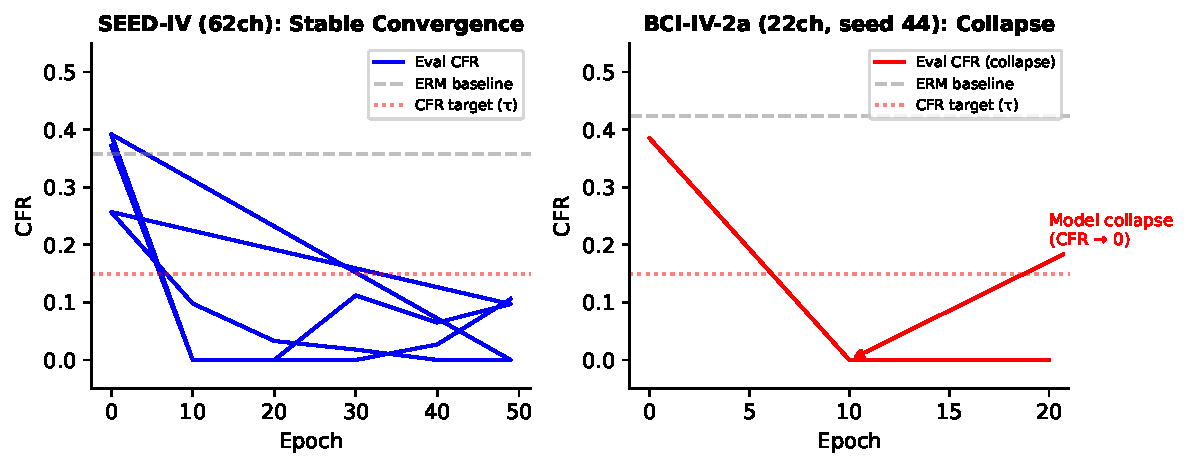
\includegraphics[width=0.85\linewidth]{figures/fig5_training_dynamics.pdf}
    \caption{NA-PGI training dynamics. \textbf{Left:} SEED-IV (62ch) shows stable CFR reduction. \textbf{Right:} BCI-IV-2a (22ch, seed 44) exhibits mid-training collapse despite adaptive $\lambda$.}
    \label{fig:dynamics}
\end{figure}

\subsection{Training Budget Comparability}

All multi-view methods (ERM-mixed, Consistency, GroupDRO, IRM, CORAL, NA-PGI) use the same number of pipeline views per batch (8 views for baselines, 256 sampled edges for NA-PGI corresponding to ${\sim}40$ unique views). Total training epochs (50) and optimizer (AdamW, lr=$10^{-3}$) are identical across methods. NA-PGI requires ${\sim}3\times$ wall-clock time due to the larger effective batch from edge sampling.

\subsection{DG Baseline Implementation Notes}

Our GroupDRO implementation uses a reweighting vector over pipeline views within each batch, but because views are randomly subsampled per batch, stable group identities are not maintained across iterations. Our CORAL implementation penalizes feature-mean divergence across pipeline views rather than full covariance alignment. These are simplified variants; canonical implementations with stable group tracking and full covariance penalties may yield different results.

% ========== end sections/appendix.tex ==========



\newpage
\section*{NeurIPS Paper Checklist}

\begin{enumerate}
\item {\bf Claims}
    \begin{enumerate}
        \item Do the main claims made in the abstract and introduction accurately reflect the paper's contributions and scope? \answerYes{See Section~\ref{sec:results} and~\ref{sec:napgi}.}
    \end{enumerate}

\item {\bf Limitations}
    \begin{enumerate}
        \item Does the paper discuss the limitations of the work performed by the authors? \answerYes{See Section~\ref{sec:discussion}, ``Limitations and failure modes.''}
    \end{enumerate}

\item {\bf Theory Assumptions and Proofs}
    \begin{enumerate}
        \item For each theoretical result, does the paper provide the full set of assumptions and a complete (and correct) proof? \answerNA{This is an empirical paper with no formal theorems.}
    \end{enumerate}

\item {\bf Experimental Result Reproducibility}
    \begin{enumerate}
        \item Does the paper fully disclose all the information needed to reproduce the main experimental results of the paper to the extent that it affects the main claims and/or conclusions of the paper? \answerYes{Section~\ref{sec:framework} specifies all preprocessing interventions, datasets, training protocol, and hyperparameters. Code will be released upon acceptance.}
    \end{enumerate}

\item {\bf Open access to data and code}
    \begin{enumerate}
        \item Does the paper provide open access to the data and code, with sufficient instructions to faithfully reproduce the main experimental results? \answerYes{All datasets are publicly available (MOABB, PhysioNet, BCMI). Code and preprocessed data will be released upon acceptance.}
    \end{enumerate}

\item {\bf Experimental Setting/Details}
    \begin{enumerate}
        \item Does the paper specify all the training and test details necessary to understand the results? \answerYes{See Section~\ref{sec:framework} and Appendix (training budget, implementation details).}
    \end{enumerate}

\item {\bf Experiment Statistical Significance}
    \begin{enumerate}
        \item Does the paper report error bars suitably and correctly? \answerYes{Table~\ref{tab:seeds} reports mean$\pm$std across 5 random seeds for NA-PGI.}
    \end{enumerate}

\item {\bf Experiments Compute Resources}
    \begin{enumerate}
        \item For each experiment, does the paper provide sufficient information on the computer resources needed to reproduce the experiments? \answerYes{See Section~\ref{sec:framework}, ``Computational cost'' paragraph.}
    \end{enumerate}

\item {\bf Code Of Ethics}
    \begin{enumerate}
        \item Does the research conducted in the paper conform, in every respect, with the NeurIPS Code of Ethics? \answerYes{}
    \end{enumerate}

\item {\bf Broader Impacts}
    \begin{enumerate}
        \item Does the paper discuss both potential positive societal impacts and negative societal impacts of the work performed? \answerYes{Our work improves reliability of EEG-based systems. No negative societal impacts are anticipated beyond standard dual-use concerns with brain-computer interfaces.}
    \end{enumerate}

\item {\bf Safeguards}
    \begin{enumerate}
        \item Does the paper describe safeguards that have been put in place for responsible release of data or models that have a high risk for misuse? \answerNA{No high-risk data or models are released.}
    \end{enumerate}

\item {\bf Licenses for existing assets}
    \begin{enumerate}
        \item Are the creators or original owners of assets used in the paper properly credited? \answerYes{All datasets are cited. MOABB, PhysioNet, and BCMI dataset licenses permit research use.}
    \end{enumerate}

\item {\bf New Assets}
    \begin{enumerate}
        \item Are new assets introduced in the paper well documented and is the documentation provided alongside the assets? \answerYes{Code and preprocessed 128-pipeline data will be released with documentation upon acceptance.}
    \end{enumerate}

\item {\bf Crowdsourcing and Research with Human Subjects}
    \begin{enumerate}
        \item For crowdsourcing experiments and research with human subjects, does the paper include the full text of instructions given to participants and details of compensation? \answerNA{No crowdsourcing or new human-subjects research. All EEG data comes from existing public datasets with prior ethical approval.}
    \end{enumerate}

\item {\bf Institutional Review Board (IRB) Approvals or Equivalent for Research with Human Subjects}
    \begin{enumerate}
        \item Does the paper describe potential risks incurred by study participants? \answerNA{We use only existing public datasets.}
    \end{enumerate}
\end{enumerate}

\end{document}
